\documentclass{beamer}
\usetheme{metropolis}
\title{Modular C++ Frameworks for Ray-Propagation}
\date{\today}
\author{J. C. Hanson (CCAPP, The Ohio State University)}
\institute{CCAPP @ OSU}
\usepackage{outlines}
\usepackage{enumitem}
\usepackage{graphicx}
\usepackage{amsmath}
\usepackage{hyperref}
\setenumerate[1]{label=\Roman*.}
\setenumerate[2]{label=\Alph*.}
\setenumerate[3]{label=\roman*.}
\setenumerate[4]{label=\alph*.}
\newcommand{\sign}{\text{sgn}}

\begin{document} \maketitle

\begin{frame}{Modular C++ Frameworks for Ray-Propagation}
\begin{outline}[enumerate]
\1 Collaboration with Dave Seckel (ARA), Robert Lahmann (ARIANNA)
\1 Problem Setup
\1 The Code
\1 Some Graphs
\end{outline}
\end{frame}

\begin{frame}{Modular C++ Frameworks for Ray-Propagation}
\small
Challenge: Speed up ray-tracing, while incorporating what we know about horizontal propagation.
\begin{outline}[enumerate]
\1 There are several approaches
\2 Use MATLAB to code up simple models to understand the physics
\2 AraSim RayTrace.h: 900 lines of code using Boost C++, index fits only
\2 A simple set of interdependent C++ classes (modular approach)
\1 Modular approach allows addition of new physics
\2 Index data versus depth
\2 Diffuse scattering vs. specular
\2 Reflective layers
\end{outline}
\end{frame}

\begin{frame}{Modular C++ Frameworks for Ray-Propagation, Ice, Reflections, RF emitters}
\small
Problem setup: (dots refer to $d/dz$, $\alpha$ with respect to horizontal)
\begin{align}
n(z)\cos(\alpha(z)) &= const \\
c_0 &= n c \\
\dot{\alpha} &= \frac{\cos\alpha}{\sin\alpha}\frac{\dot{n}}{n} \\
dz &= c dt \sin\alpha \\
\frac{d\alpha}{dt} &= \cos\alpha \frac{c_0}{n^2} \frac{dn}{dz}
\end{align}
Knowing how the angle depends on time, we know how to increment it, and (x,z).  Also, Robert Lahmann has shown how this approach falls out of my Fermat's Principle approach, which is informative.
\end{frame}

\begin{frame}{The code}
clone from github.com:
\url{https://github.com/918particle/Ray_Propagation}
\begin{itemize}
\item Minimal octave example: \texttt{Ray\_Propagation/code/RayProp\_jch.m}
\item With diffuse scattering and reflective surfaces: coming soon
\item C++ modules: \texttt{Ray\_Propagation/code/cpp\_propagation}
\end{itemize}
\end{frame}

\begin{frame}{The code}
The C++ module has four classes:
\begin{itemize}
\item Emitter.h: Handles the position and angle of the ray within (x,z) coordinate system
\item Ice.h: Handles index of refraction profile, attenuation length profile, cylindrical coordinates
\item Reflector.h: Defines depths at which reflectors exist (will get this from Ice.h soon)
\item Propagator.h: Handles propagation using differential approach, obtains $n(z)$ from Ice.h
\end{itemize}
\end{frame}

\begin{frame}{Octave implementation (no reflections or diffuse scattering)}
\begin{center}
\includegraphics[width=0.5\textwidth]{figures/April28_plot1.pdf}
\includegraphics[width=0.5\textwidth]{figures/April28_plot2.pdf}
\end{center}
\end{frame}

\begin{frame}{Octave implementation (no reflections or diffuse scattering)}
\begin{center}
\includegraphics[width=0.5\textwidth]{figures/April28_plot5.pdf}
\includegraphics[width=0.5\textwidth]{figures/April28_plot6.pdf}
\end{center}
\end{frame}

\begin{frame}{C++ modular implementation (no reflections or diffuse scattering)}
\begin{center}
\includegraphics[width=0.5\textwidth,angle=270]{figures/May11_plot1.eps}
\end{center}
\end{frame}

\begin{frame}{Coming soon: Spoorti }
\small
Challenge: Speed up ray-tracing, while incorporating what we know about horizontal propagation.
\begin{outline}[enumerate]
\1 There are several approaches
\2 Use MATLAB to code up simple models to understand the physics
\2 AraSim RayTrace.h: 900 lines of code using Boost C++, index fits only
\2 A simple set of interdependent C++ classes (modular approach)
\1 Modular approach allows addition of new physics
\2 Index data versus depth
\2 Diffuse scattering vs. specular
\2 Reflective layers
\end{outline}
\end{frame}


\end{document}
